\documentclass[border=10pt]{standalone}

\usepackage{tikz}
\usepackage{tikzsymbols}
\usetikzlibrary{calc,patterns,shapes.geometric}

\def\centerarc[#1](#2)(#3:#4:#5){\draw[#1] ($(#2)+({#5*cos(#3)},{#5*sin(#3)})$) arc (#3:#4:#5);}

\begin{document}
	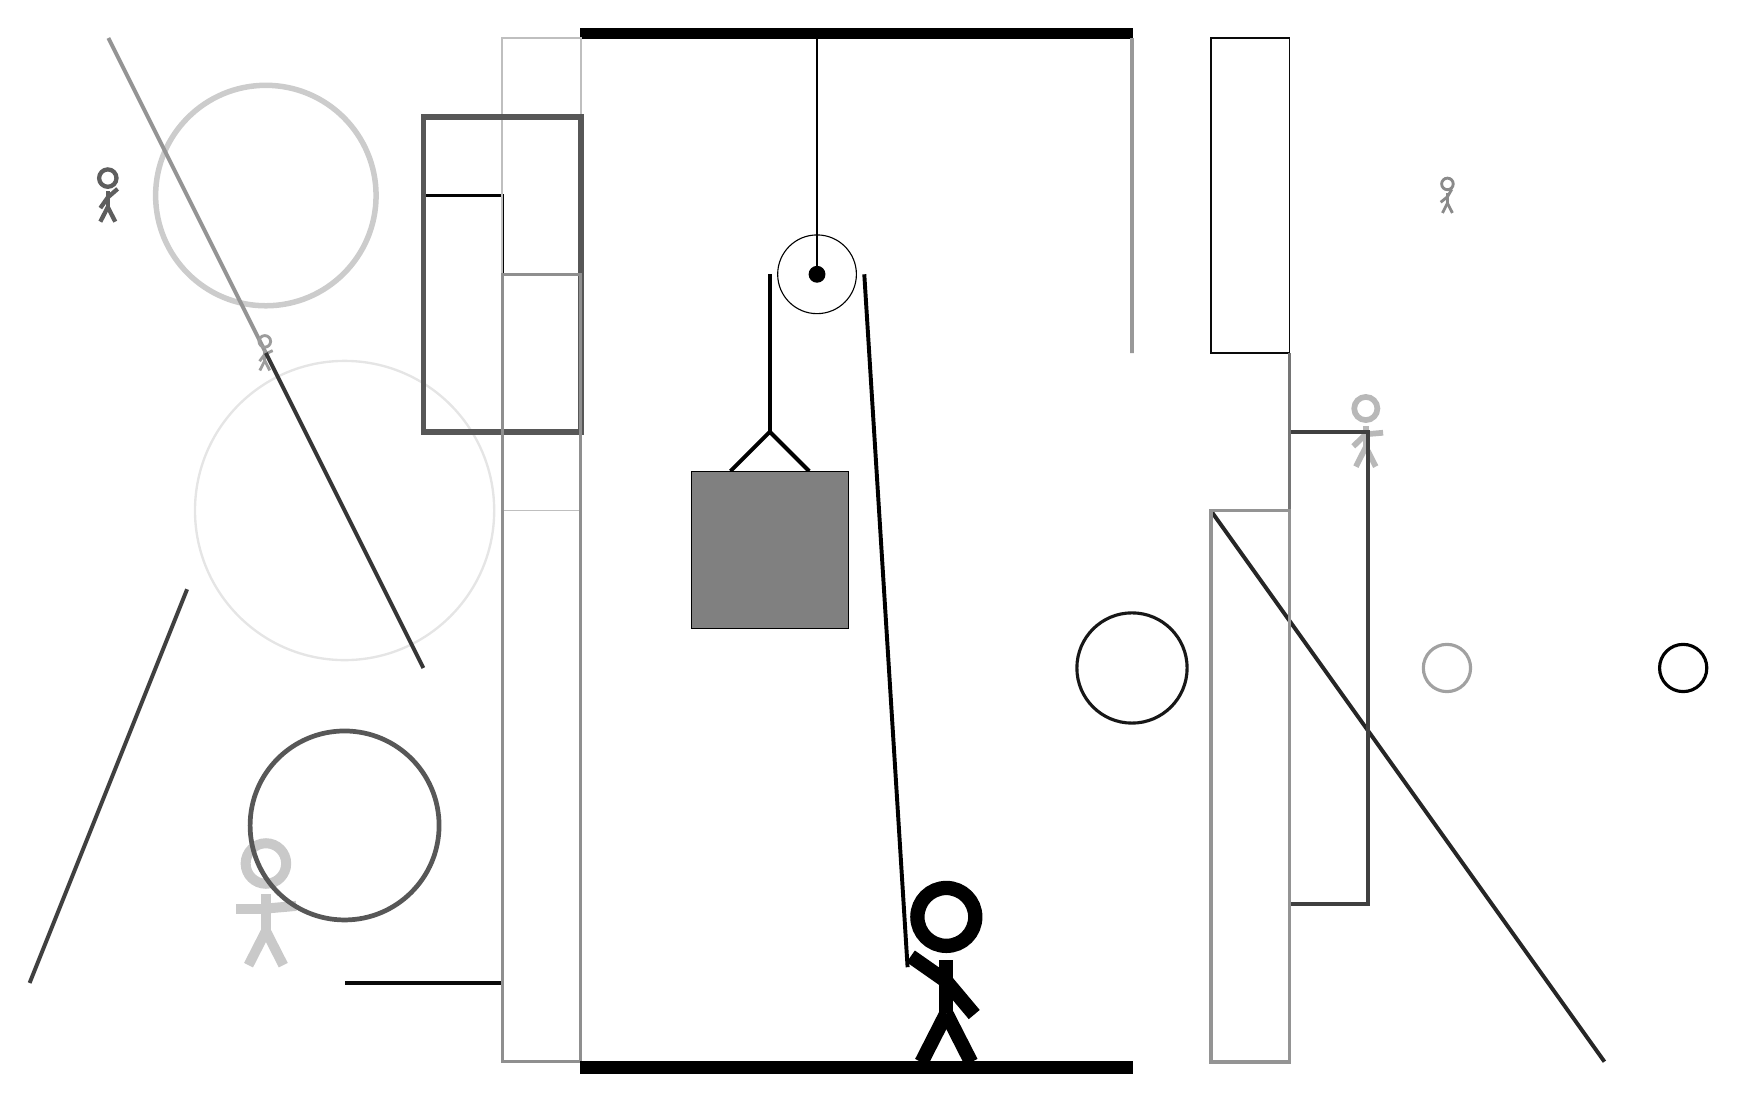
\begin{tikzpicture}
		%%%%% START %%%%%
		
		\draw[fill=black] (-2, 10) rectangle (5, 10.125);
		
		\draw (1, 7) circle (0.5);
		\draw[fill=black] (1, 7) circle (0.1);
		\draw (1, 10) -- (1, 7);
		
		\draw[line width=0.5mm, color=black!85](6, 4) -- (11, -3);
		
		\draw[line width=0.2mm, color=black!96] (7, 10) rectangle (6, 6);
		\draw[line width=0.4mm, color=black!99] (-3, 8) rectangle (-4, 5);
		\node[line width=0.6mm, color=black!28] at (8, 5) {\Strichmaxerl[4][44][5]};
		\draw [line width=0.7mm, color=black!20](-6, 8) circle (1.4);
		\draw[line width=0.5mm, color=black!75] (7, -1) rectangle (8, 5);
		\draw[line width=0.5mm, color=black!42](-6, 6) -- (-8, 10);
		
		\draw[line width=0.5mm, color=black!96](-3, -2) -- (-5, -2);
		\draw[line width=0.5mm, color=black!75](-7, 3) -- (-9, -2);
		\draw [line width=0.4mm, color=black!100](12, 2) circle (0.3);
		
		\node[line width=0.4mm, color=black!39] at (-6, 6) {\Strichmaxerl[2][53][25]};
		\draw [line width=0.3mm, color=black!10](-5, 4) circle (1.9);
		\draw [line width=0.4mm, color=black!37](9, 2) circle (0.3);
		
		\draw[line width=0.4mm, color=black!40] (5, 10) rectangle (5, 6);
		\draw[line width=0.2mm, color=black!25] (-2, 4) rectangle (-3, 10);
		\draw[line width=0.7mm, color=black!66] (-2, 9) rectangle (-4, 5);
		
		\draw[line width=0.5mm, color=black!54] (7, 6) rectangle (7, -1);
		
		\node[line width=0.5mm, color=black!21] at (-6, -1) {\Strichmaxerl[7][0][5]};
		\draw[line width=0.5mm, color=black!79](-4, 2) -- (-6, 6);
		\draw [line width=0.6mm, color=black!66](-5, 0) circle (1.2);
		\node[line width=0.3mm, color=black!63] at (-8, 8) {\Strichmaxerl[3][55][41]};
		
		\draw[line width=0.4mm, color=black!44] (-2, -3) rectangle (-3, 7);
		\draw [line width=0.4mm, color=black!91](5, 2) circle (0.7);
		\node[line width=0.2mm, color=black!46] at (9, 8) {\Strichmaxerl[2][39][60]};
		\draw[line width=0.5mm, color=black!42] (7, -3) rectangle (6, 4);
		
		
		\draw[line width=0.5mm] (-0.1, 4.5) -- (0.4, 5.0) -- (0.9, 4.5);
		\draw[fill=black!50] (-0.6, 4.5) rectangle (1.4, 2.5);
		
		\draw[line width=0.5mm] (0.4, 7) -- (0.4, 5.0);
		\centerarc[line width=0.5mm](1, 7)(0:180:0.6);
		\draw[line width=0.5mm](1.6, 7) -- (2.15, -1.8);
		
		\node at (2.6, -1.9) {\Strichmaxerl[10][-35][-50]};
		
		\draw[fill=black] (-2, -3) rectangle (5, -3.15);
		
		%%%%% END %%%%%
	\end{tikzpicture}
\end{document}